\documentclass[10pt]{article}
\usepackage[letterpaper,landscape,margin=0.65in]{geometry}
\usepackage{graphicx}
\usepackage{booktabs}
\usepackage{amsmath}
\usepackage[T1]{fontenc}
\usepackage{hyperref}
\hypersetup{pdftitle={FROB C5 exact quotient matrix factor kernels},
  pdfsubject={EXP-FROB-91ee9c; matrix-model C5 theorem; historical execution review open}}
\setlength{\parindent}{0pt}
\setlength{\parskip}{0.45em}
\title{FROB C5 exact quotient matrix factor kernels}
\author{Validation audit, 22 October 2026}
\date{}
\begin{document}
\maketitle
\vspace{-2em}

\textbf{Scope.} The frozen \texttt{RUN-FROB-91ee9c-7119f2} core cells have
three previously certified $5\times5$ quotient-basis $q$-power matrices.
This target evaluates their nontrivial cyclotomic factor polynomials and their
five-term trace polynomials as linear maps over the base fields.

\begin{center}
\begin{tabular}{llll}
\toprule
Base field & Nontrivial factors & Lean matrix result & Trace-kernel dimension \\
\midrule
$\mathbf F_{11}$ & four distinct linears & successive direct sum $=\ker T$ & 4 \\
$\mathbf F_{13}$ & one irreducible quartic & factor kernel $=\ker T$ & 4 \\
$\mathbf F_{19}$ & two irreducible quadratics & direct sum $=\ker T$ & 4 \\
\bottomrule
\end{tabular}
\end{center}

\textbf{Proof.} The exact matrix entries were proved from frozen quotient
moduli in a separate Lean certificate. The present source computes
$M_q^5=I$ and $T_q=I+M_q+M_q^2+M_q^3+M_q^4$ for each $q$.
It factors each trace matrix as a rank-one diagonal matrix times an
invertible upper-triangular matrix. Rank-nullity gives $\dim\ker T_q=4$.
Previously checked polynomial factorizations and coprimality give the direct
factor-kernel sums, instantiated here with \texttt{Matrix.toLin'} of the
exact frozen matrices. All three statements are combined in one target theorem.

\textbf{Machine verification.} Lean source commit \texttt{458c91dbdcb8}
uses pinned Lean 4.35.0-rc1. The exact-source verifier passed an 8,973-job full build and 3,097-job
target build. Its global audit found 647 theorem declarations with standard
axioms only; the requested theorem audit passed. Independent semantic review
remains pending.

\textbf{Boundary.} This closes the mathematical C5 factor-kernel calculation
for the three exact recorded matrices. A full-map q-power representation lemma,
historical Sage implementation refinement, original run source custody,
independent code review, C8 and the full experiment success gate remain open. No experiment was rerun and no
performance dashboard value changed.

\newpage
\begin{center}
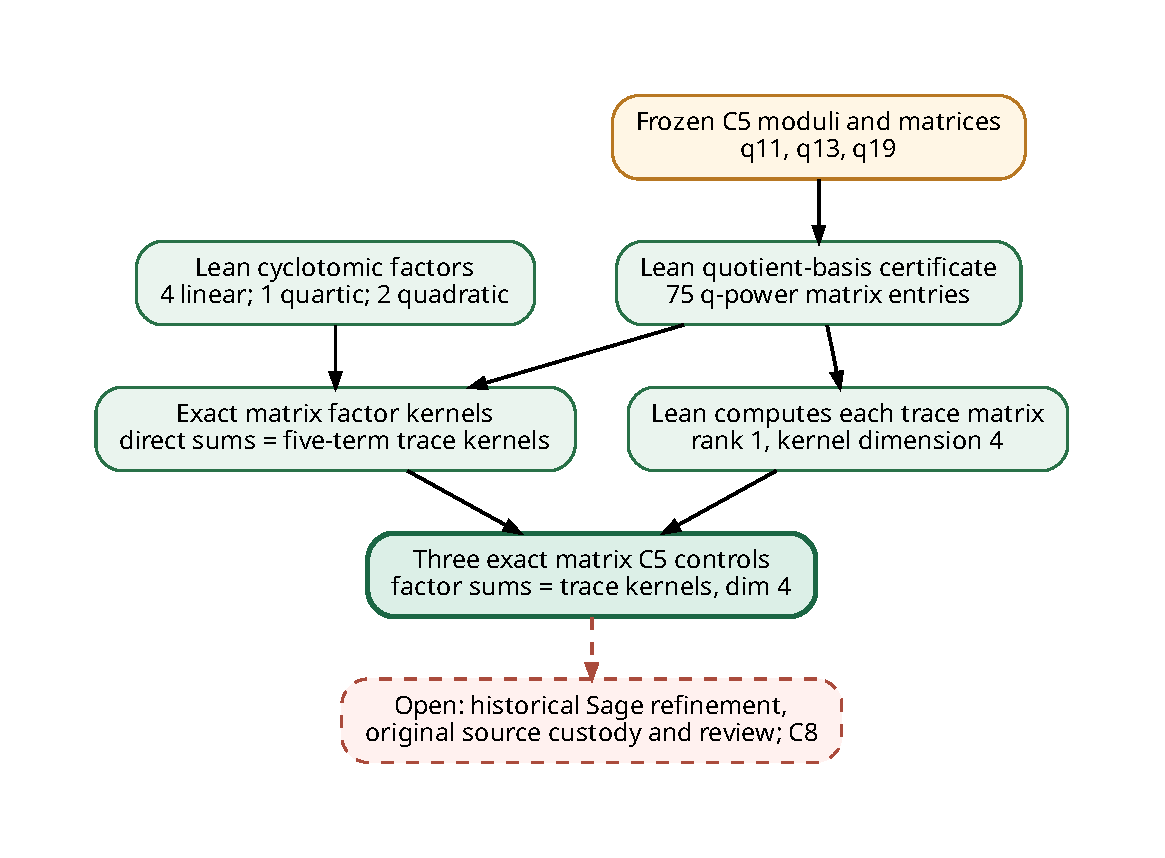
\includegraphics[width=\textwidth,height=0.82\textheight,keepaspectratio]{proof-figure.pdf}
\end{center}
\end{document}
